\documentclass{beamer}
% Remove [handout] for pause to work.
\usetheme{metropolis}

\usepackage{graphicx}
\graphicspath{{images/}}

\colorlet{shade}{gray!40}

\DeclareMathOperator{\Ad}{Ad}
\DeclareMathOperator{\cdf}{cdf}
\DeclareMathOperator{\D}{D}
\DeclareMathOperator{\GL}{GL}
\DeclareMathOperator{\h}{H}
\DeclareMathOperator{\N}{N}
\DeclareMathOperator{\R}{R}
\DeclareMathOperator{\rk}{rk}
\DeclareMathOperator{\ram}{ram}
\DeclareMathOperator{\sgn}{sgn}
\DeclareMathOperator{\ST}{ST}
\DeclareMathOperator{\SU}{SU}
\DeclareMathOperator{\sym}{sym}
\DeclareMathOperator{\tr}{tr}
\DeclareMathOperator{\X}{X}
\newcommand{\bC}{\mathbf{C}}
\newcommand{\bF}{\mathbf{F}}
\newcommand{\bQ}{\mathbf{Q}}
\newcommand{\bR}{\mathbf{R}}
\newcommand{\bZ}{\mathbf{Z}}
\newcommand{\dd}{\mathrm{d}}
\newcommand{\frob}{\mathrm{fr}}

\newtheorem{conjecture}{Conjecture}

\title{Counterexamples related to the Sato--Tate conjecture}
\author{Daniel Miller}
\institute{Cornell University}
\date{25 April 2017}





% Outline:
% Motivation: 
%  - What is the problem I'm trying to solve?
%    2 problems: does RH => AT? is there a Galois proof of ST?
%  - Why is this problem interesting or important?
%    * AT=>RH: so far proofs of ST have proved things about L-functions. 
%      How far can knowledge of L-functions take you?
%    * Galois ST: does ST conjecture follow from Galois theory alone? 
%  - Why is my solution interesting?
%    * Two "No!" answers. 
%    * Proving AT will take more than just L-functions.
%    * ST fundamentally involves automorphy!
% Work
%  - What theorems have I proved? 
%    * "Master Galois theorem"
%    * "dioph approx counterexample"
% Related work
%  - Who else has attacked this problem or similar problems? 
%    * Pande, KLR, Thorner, Mazur
%  - In what ways is my solution better? 
%    * Better than Pande: stronger results
%    * convenient "packaging" of KLR
%    * shows that Thorner doesn't generalize to CM
%  - In what ways is it limited? 
%    * only addresses CM varieties - may not work for SU(2)
% So what?
%  - need new directions to prove AT, even for CM case. 
%  

% Sasha feedback:
% Go slower
% Include some computations / pretty pictures
% Give more background & perspective. How do my results fit in the big picture?

% Ivy feedback:
% Don't raise tone of voice at the end of each sentence!





\begin{document}

\begin{frame}
\titlepage
\end{frame}



\begin{frame}
\frametitle{Outline}
\tableofcontents
\end{frame}





\section{Motivation and background}

\begin{frame}{Sato--Tate conjecture}
$E_{/\bQ}$ non-CM elliptic curve, $l$ prime, $\rho_l\colon G_\bQ \to \GL_2(\bZ_l)$. 
\pause

\textbf{Fact:}
$a_p = \tr\rho_l(\frob_p) = p+1 - \# E(\bF_p)$, 
\pause
$|a_p|\leqslant 2\sqrt p$. 
\pause
(Hasse) % proved in 1930s
\pause

Satake parameter: $\theta_p = \cos^{-1}\left( \frac{a_p}{2\sqrt p}\right)$. 
\pause

Sato--Tate measure: $\ST = \frac{2}{\pi} \sin^2 \theta$ 
\pause
% "natural" = space of conjugacy classes (Serre's notation)
(Haar measure on $\SU(2)^\natural$). 
\pause

% Sato--Tate conjecture. See "Algebraic cycles and poles of zeta functions"
% 1965 for first statement in print.
% Proved by Barnet--Lamb, Geraghty, Harris, Shepherd--Barron, Taylor
\begin{theorem}[Barnet-Lamb--Geraghty--Harris--Taylor]
$\{\theta_p\}$ is $\ST$-equidistributed. 
\end{theorem}
\pause

Quantify rate of convergence of 
$\frac{1}{\pi(N)} \sum_{p\leqslant N} \delta_{\theta_p}$ to $\ST$. 
\pause

% Nikolai Smirnov
% Andrey Kolmogorov
Use discrepancy (Kolmogorov--Smirnov statistic). 
\end{frame}



\begin{frame}{Akiyama--Tanigawa conjecture}
\[
	D_N = \sup_{x\in [0,\pi]}\left| \frac{1}{\pi(N)} \sum_{p\leqslant N} 1_{[0,x)}(\theta_p) - \int 1_{[0,x)}(\theta) \, \dd\ST(\theta)\right| .
\]
\pause

\begin{conjecture}[Akiyama--Tanigawa]
$D_N \ll N^{-\frac 1 2 + \epsilon}$. 
\end{conjecture}
\pause

There is a variant of this conjecture for CM elliptic curves.
\pause
Also for CM abelian varieties, 
\pause
even motives.
\pause

\begin{theorem}[Akiyama--Tanigawa]
Akiyama--Tanigawa conjecture $\Rightarrow$ Riemann hypothesis for $E$.
\end{theorem}
\pause

\begin{theorem}[Mazur]
Akiyama--Tanigawa conjecture $\Rightarrow$ Riemann hypothesis for $\sym^k E$
\end{theorem}
\end{frame}



\begin{frame}{Computational evidence}
\begin{center}
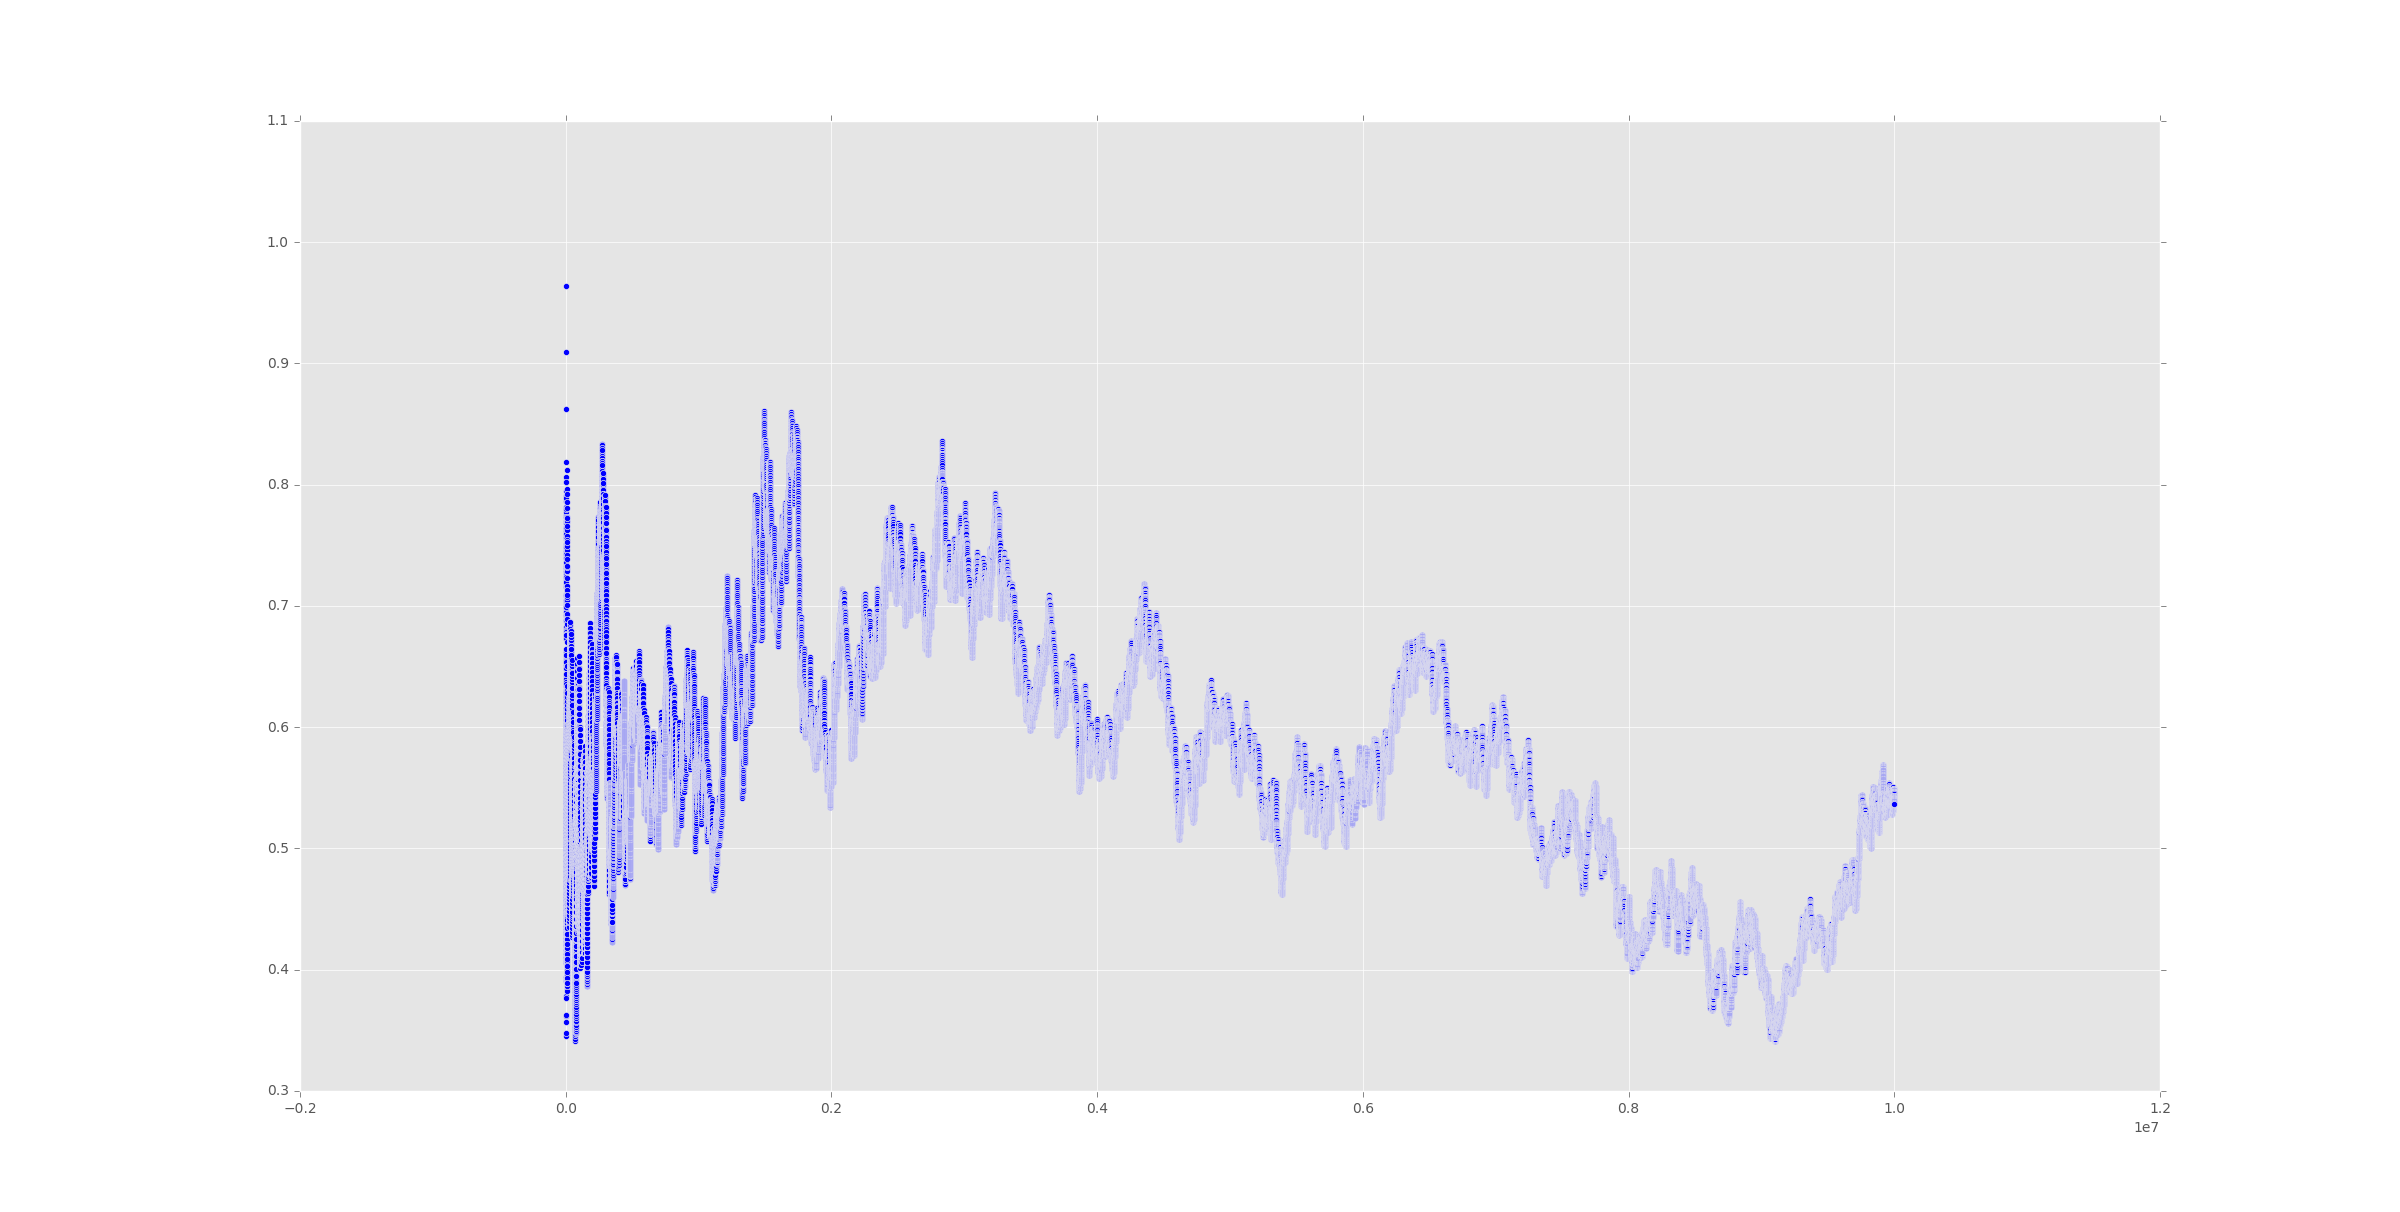
\includegraphics[width=\textwidth]{11a1}

$\sqrt{\pi(N)} \cdot \D_N$ for $y^2 + y = x^3 - x$, $N\leqslant 10^7$.
\end{center}
\end{frame}



\begin{frame}{Related results}
% Alina Bucar & Kiran Kedlaya. 
% "an application of the effective Sato--Tate conjecture"
\textbf{Theorem (Bucar--Kedlaya).}
Assume analytic continuation of $L(\sym^k E,s)$, GRH, and functional equation 
for all $k\geqslant 1$. Then $\D_N \ll N^{-\frac 1 4+\epsilon}$. 
\pause

% Jeremy Rouse and Jesse Thorner.
% "the explicit Sato--Tate conjecture and densities pertaining to 
% Lehmer-type questions"
\textbf{Theorem (Rouse--Thorner).}
Same result (with explicit constants) for a modular form of arbitrary weight	. 
\pause

% Harald Niederreiter.
% "the distribution of values of Kloosterman sums"
\textbf{Theorem (Niederreiter).}
Let $E_{/F}$, where $F$ is a function field. Then 
$\D_N \ll N^{-\frac 1 4+\epsilon}$. 
\pause

% Zev Rosengarten
% "an Erdos--Turan inequality for compact simply-connected semisimple Lie groups"
\textbf{Theorem (Rosengarten).}
For $G = \ST(M)$ semisimple, GRH $\Rightarrow\D_N \ll N^{-\alpha_G+\epsilon}$, 
where $\alpha_G\to 0$ as $\rk G\to \infty$. 
\pause

\textbf{Common ingredient.}
Erd\"os--Tur\'an inequality: from a bound on
$\left|\sum_{p\leqslant N} \tr \rho(x_p)\right|$ to a bound on $\D_N$.
\end{frame}



\begin{frame}{Context}
\textbf{Question.} 
Is the Sato--Tate conjecture a Galois-theoretic result?
\pause

\begin{theorem}[Pande]
Let $\epsilon>0$. Then there exists an infinitely ramified representation 
$\rho\colon G_\bQ \to \GL_2(\bZ_l)$ such that $\theta_p\in B_\epsilon(\pi/2)$ 
for a density one set of primes. 
\end{theorem}
\pause

\begin{theorem}[Khare--Rajan]
Any $\rho\colon G_\bQ \to \GL_2(\bZ_l)$ is ramified at a density zero set of 
primes. 
\end{theorem}
\pause

\textbf{Question (Serre).} Can you control the growth of 
$\pi_{\ram(\rho)}(x)$?
\pause

\textbf{Answer (Khare--Larsen--Ramakrishna).} No!
\end{frame}



\begin{frame}{Questions}
\textbf{Q1.} Can Pande's results be strengthened to yield equidistribution? 
\pause

\textbf{Q2.} If so, can the measure be specified?
\pause

\textbf{Q3.} Can the rate of convergence of empirical measures to the true measure 
be specified?
\pause

\textbf{Q4.} Can the growth of $\pi_{\ram(\rho)}(x)$ be controlled?
\pause

\textbf{Q5.} Can anything be said about the $L$-functions associated with $\rho$?
\pause

\textbf{Answer.} Yes! to Q1--Q5. 
\end{frame}





\section{Discrepancy and Dirichlet series}

\begin{frame}{Discrepancy}
\begin{definition}
Let $\{\theta_p\}$ be a sequence in $[0,\pi]$, $\mu$ a measure on $[0,\pi]$. 
The \emph{discrepancy} is 
\[
	\D_N(\{\theta_p\},\mu) =  \sup_{x\in [0,\pi]}\left| \frac{1}{\pi(N)} \sum_{p\leqslant N} 1_{[0,x)}(\theta_p) - \int 1_{[0,x)}(\theta) \, \dd\mu(\theta)\right| .
\]
\end{definition}
\pause

\textbf{Fact.}
$\{\theta_p\}$ are $\mu$-equidistributed if and only if $D_N \to 0$. 
\pause

\textbf{Fact.}
$\frac{\log N}{N} \ll D_N$. The \emph{van der Corput sequence} achieves this. 
% and there's a "trick" to get the same rate of decay of discrepancy for any 
% absolutely continuous measure.
\end{frame}



\begin{frame}{Dirichlet series}
\begin{definition}
For $k\geqslant 1$, 
\[
	L(\sym^k \rho,s) = \prod_p \det\left( 1 - \sym^k \left(\begin{smallmatrix} e^{i \theta_p} & 0\\ 0 & e^{-i \theta_p}\end{smallmatrix}\right) p^{-s}\right)^{-1}
\]
\end{definition}
\pause

\begin{definition}
For $f\colon [0,\pi] \to \bC$ of bounded variation with $\mu(f) = 0$,  
\[
	L_f(s) = \prod_p \left( 1 - f(\theta_p) p^{-s}\right)^{-1}
\]
\end{definition}
\pause

\textbf{Example (Ramakrishna).}
$L_{\sgn}(s) = \prod_p \left(1 - \sgn(a_p) p^{-s}\right)^{-1}$. 
\end{frame}



\begin{frame}{Dirichlet series---basic facts}
\begin{theorem}[M.]
If $\left| \sum_{p\leqslant N} f(\theta_p)\right| \ll N^{\alpha+\epsilon}$, 
then $L_f(s)$ admits a nonvanishing analytic continuation to $\Re > \alpha$. 
\end{theorem}
\pause

\begin{corollary}
If $D_N \ll N^{\alpha-1+\epsilon}$, then $L_f(s)$ admits a nonvanishing 
analytic continuation to $\Re > \alpha$. 
\end{corollary}
\pause

\begin{definition}
$U_k(\theta) = \frac{\sin((k+1)\theta)}{\sin\theta} = \tr\sym^k \left(\begin{smallmatrix} e^{i \theta_p} & 0\\ 0 & e^{-i \theta_p}\end{smallmatrix}\right)$.
\end{definition}
\pause

\begin{theorem}
If $\left| \sum_{p\leqslant N} U_k(\theta_p)\right| \ll N^{\alpha+\epsilon}$, 
then $L(\sym^k\rho, s)$ admits a nonvanishing analytic continuation to 
$\Re > \alpha$. 
\end{theorem}
\end{frame}





\section{Main theorem}

\begin{frame}{Ingredients}
1. Fix a rational prime $l\geqslant 5$. 
\pause

2. Fix an odd, absolutely irreducible, weight 2 representation 
$\bar\rho\colon G_\bQ \to \GL_2(\bF_l)$.
\pause
\textcolor{blue}{$\rho$ will be a lift of $\bar\rho$.}
\pause

3. Fix a function $h\colon \bR^+ \to \bR_{\geqslant 1}$ which increases slowly 
to infinity. 
\pause
\textcolor{blue}{We will have $\pi_{\ram(\rho)}(x) \ll h(x)$.}
\pause

4. Fix an absolutely continuous probability measure $\mu$ on $[0,\pi]$, with 
probability density function $f(\theta)\ll \sin\theta$.
\pause
\textcolor{blue}{The angles $\{\theta_p\}$ will be $\mu$-equidistributed.}
\pause

5. Fix $\alpha\in \left(0,\frac 1 3\right)$. 
\pause
\textcolor{blue}{The discrepancy will decay like $\pi(N)^{-\alpha}$.}
\end{frame}



\begin{frame}{Questions}
\textbf{Q1.} Can Pande's results be strengthened to yield equidistribution? 

\textbf{Q2.} If so, can the measure be specified?

\textbf{Q3.} Can the rate of convergence of empirical measures to the true measure 
be specified?

\textbf{Q4.} Can the growth of $\pi_{\ram(\rho)}(x)$ be controlled?

\textbf{Q5.} Can anything be said about the $L$-functions associated with $\rho$?
\end{frame}



\begin{frame}{Main theorem}
\begin{theorem}[M.]
Let $l$, $\bar\rho$, $h$, $\mu$, and $\alpha$ be as above. Then there exists 
$\rho\colon G_\bQ \to \GL_2(\bZ_l)$ such that 
\pause
\begin{enumerate}
\item
$\rho \equiv \bar\rho\pmod{l}$. 
\pause

\item
$\pi_{\ram(\rho)}(x) \ll h(x)$. 
\pause
\textcolor{blue}{(Yes to Q4. 
\pause
$\log x$, 
\pause
$\log^{10^{10}}x$, 
\pause
$A^{-1}(x)$)}
\pause

\item
For each unramified $p$, $a_p = \tr \rho(\frob_p)\in \bZ$ and satisfies the 
Hasse bound.
\pause

\item
$\D_N(\{\theta_p\},\mu) = \Theta(\pi(N)^{-\alpha})$. 
\pause
\textcolor{blue}{(Yes to Q1--Q3.)}
\pause

\item
If $(\theta\mapsto \pi-\theta)_\ast \mu = \mu$, then for each odd $k$, 
$L(\sym^k \rho,s)$ satisfies the Riemann hypothesis. 
\pause
\textcolor{blue}{(Yes to Q5.)}
\end{enumerate}
\end{theorem}
\end{frame}






\section{Sketch of proof}

\begin{frame}{Overview}
1. Prove the theorem for $a_p$ not coming from a Galois representation. 
\pause

2. Construct $\rho$ with $\tr\rho(\frob_p)$ close to the choices from 1. 
\pause

3. Control the growth $\pi_{\ram}(x)$. 
\pause

4. Inductive process.
\pause

5. Riemann hypothesis for $L(\sym^k\rho,s)$, $k$ odd.
\end{frame}



\begin{frame}{Overview}
\textcolor{blue}{
1. Prove the theorem for $a_p$ not coming from a Galois representation.}

\color{shade}
2. Construct $\rho$ with $\tr\rho(\frob_p)$ close to the choices from 1. 

3. Control the growth $\pi_{\ram}(x)$. 

4. Inductive process.

5. Riemann hypothesis for $L(\sym^k\rho,s)$, $k$ odd.
\end{frame}



\begin{frame}{Prescribing discrepancy decay}
\begin{theorem}[M.]
If $\alpha\in \left(0,\frac 1 3\right)$, there exists a sequence 
$(x_2,x_3,x_5,\dots)$ in $[-1,1]$ such that 
$| D_N - \pi(N)^{-\alpha}| \ll \pi(N)^{-1}$. 
\end{theorem}
\pause

(Can have $x_p = \frac{a_p}{2\sqrt p}$ for $a_p\in \bZ$ satisfying the 
Hasse bound.) 
\pause

\textbf{Fact:} 
Discrepancy is invariant under pushforward by $\cos$ and $\cos^{-1}$. 
\pause

\textbf{Idea}:
Construct $\rho$ so that $\frac{a_p}{2\sqrt p}\approx x_p$. 
\pause

\textbf{Fact:} 
If $(x_p^{(1)})$ is a sequence with $|x_p - x_p^{(1)}| \ll p^{-\frac 1 2+\epsilon}$, 
then $\D_N^{(1)} = \Theta(\pi(N)^{-\alpha})$. 
\end{frame}



\begin{frame}{Overview}
\color{shade}
1. Prove the theorem for $a_p$ not coming from a Galois representation.

\textcolor{blue}{
2. Construct $\rho$ with $\tr\rho(\frob_p)$ close to the choices from 1.}

3. Control the growth $\pi_{\ram}(x)$. 

4. Inductive process.

5. Riemann hypothesis for $L(\sym^k\rho,s)$, $k$ odd.
\end{frame}



\begin{frame}{Lifting Galois representations}
Construct $\rho$ as $\varprojlim \rho_n$, where 
$\rho_n\colon G_{\bQ,R_n} \to \GL_2(\bZ/l^n)$.
\pause

For all $n$, require $\det\rho_n \equiv \kappa\pmod{l^n}$
\pause
($l$-adic cyclotomic character)
\pause

Passage from $\rho_n$ to $\rho_{n+1}$ is governed by 
$\h^i(G_{\bQ,R_n},\Ad^0\bar\rho)$, $i = 1,2$.
\pause

\begin{theorem}[Khare--Larsen--Ramakrishna]
Fix a finite set $U$ of primes. Then there exists a finite set $N$ of primes 
such that 
\[
	\h^1(G_{\bQ,R_n\cup N},\Ad^0\bar\rho) \xrightarrow{\sim}\prod_{p\in R_n} \h^1(G_{\bQ_p}, \Ad^0\bar\rho) \times \prod_{p\in U} \h_\mathrm{nr}^1(G_{\bQ_p},\Ad^0\bar\rho)
\]
\end{theorem}

\textbf{Corollary.}
Given $\rho_n\colon G_{\bQ,R_n} \to \GL_2(\bZ/l^n)$, can choose 
$\tr\rho_{n+1}(\frob_p)$ for all $p$ in a finite set.
\pause
\textcolor{blue}{(Finitely many more ramified primes.)}
\end{frame}



\begin{frame}{Overview}
\color{shade}
1. Prove the theorem for $a_p$ not coming from a Galois representation.

2. Construct $\rho$ with $\tr\rho(\frob_p)$ close to the choices from 1.

\textcolor{blue}{
3. Control the growth $\pi_{\ram}(x)$.}

4. Inductive process.

5. Riemann hypothesis for $L(\sym^k\rho,s)$, $k$ odd.
\end{frame}



\begin{frame}{Controlling ramified primes}
Given $\rho_n\colon G_{\bQ,R_n} \to \GL_2(\bZ/l^n)$ and choices of 
$\tr \rho_{n+1}(\frob_p)\pmod{l^{n+1}}$, need to add finite set $N$ to 
$R_n$. 
\pause

Each $p\in N$ is chosen from a positive-density set of primes.
\pause

So $p$ can be arbitrarily large!
\pause

If $\pi_R(x) \leqslant h(x)\,(\forall x)$, can force this for 
$\pi_{R\cup N}(x)$. 
\pause

$\pi_{\ram(\bar\rho)}(x)\leqslant h(x)$ may not hold---scale $h$ to make this 
true!
\pause

\textbf{Fact:} constant in $\pi_{\ram(\rho)}(x) \ll h(x)$ only depends on 
\textcolor{blue}{$\bar\rho$}. 
\end{frame}



\begin{frame}{Overview}
\color{shade}
1. Prove the theorem for $a_p$ not coming from a Galois representation.

2. Construct $\rho$ with $\tr\rho(\frob_p)$ close to the choices from 1.

3. Control the growth $\pi_{\ram}(x)$. 

\textcolor{blue}{
4. Inductive process.}

5. Riemann hypothesis for $L(\sym^k\rho,s)$, $k$ odd.
\end{frame}



\begin{frame}{Lifting Galois representations---first stage}
Lift from $\bZ/l$ to $\bZ/l^2$. 
\pause

Fix a \textcolor{blue}{large} finite set $U_1$ of primes. 
\pause

For $p\in U_1$, can choose $a_p\in \bZ$ subject only to 
$|a_p|\leqslant 2\sqrt p$ and $a_p\equiv \tr\rho_1(\frob_p)\pmod{l}$. 
\pause

We can ensure 
$\left| \frac{a_p}{2\sqrt p} - x_p\right| \leqslant \frac{l}{2\sqrt p}$.
\pause

For $N\leqslant \max U_1$, $\D_N(\{\theta_p\},\mu) = \Theta(\pi(N)^{-\alpha})$. 
\pause

Make $U_1$ so large that for $p>\max U_1$, $l^2 < \log p$. 
\end{frame}



\begin{frame}{Main theorem}
\begin{theorem}[M.]
Let $l$, $\bar\rho$, $h$, $\mu$, and $\alpha$ be as above. Then there exists 
$\rho\colon G_\bQ \to \GL_2(\bZ_l)$ such that 
\begin{enumerate}
\item
$\rho \equiv \bar\rho\pmod{l}$. 

\item
$\pi_{\ram(\rho)}(x) \ll h(x)$. 

\item
For each unramified $p$, $a_p = \tr \rho(\frob_p)\in \bZ$ and satisfies the 
Hasse bound.

\item
$\D_N(\{\theta_p\},\mu) = \Theta(\pi(N)^{-\alpha})$. 

\item
If $(\theta\mapsto \pi-\theta)_\ast \mu = \mu$, then for each odd $k$, 
$L(\sym^k \rho,s)$ satisfies the Riemann hypothesis. 
\end{enumerate}
\end{theorem}
\end{frame}



\begin{frame}{Lifting Galois representations---inductive step}
Lift from $\bZ/l^n$ to $\bZ/l^{n+1}$. 
\pause

Have already chosen $a_p$ for $p\in U_n$. 
\pause
\textcolor{blue}{(1--5 hold)}
\pause

Fix a \textcolor{blue}{really huge} $U_{n+1}\supset U_n$.
\pause

For $p\in U_{n+1}\smallsetminus U_n$, can choose $a_p\in \bZ$ subject only to 
$|a_p| \leqslant 2\sqrt p$ and $a_p \equiv \tr\rho_n(\frob_p)\pmod{l^n}$. 
\pause

We can ensure 
$\left| \frac{a_p}{2\sqrt p} - x_p\right| \leqslant \frac{l^n}{2\sqrt p}$.
\pause
\textcolor{blue}{($l^n \ll \log p$)}.
\pause

For $N\leqslant \max U_{n+1}$, $\D_N(\{\theta_p\},\mu) = \Theta(\pi(N)^{-\alpha})$. 
\end{frame}



\begin{frame}{Overview}
\color{shade}
1. Prove the theorem for $a_p$ not coming from a Galois representation.

2. Construct $\rho$ with $\tr\rho(\frob_p)$ close to the choices from 1.

3. Control the growth $\pi_{\ram}(x)$. 

4. Inductive process.

\textcolor{blue}{
5. Riemann hypothesis for $L(\sym^k\rho,s)$, $k$ odd.}
\end{frame}



\begin{frame}{Riemann hypothesis}
How can we make $L(\sym^k \rho,s)$, $k$ odd, satisfy the Riemann hypothesis?
\pause

$\left|\sum_{p\leqslant N} U_k(\theta_p)\right| \ll N^{\frac 1 2+\epsilon}$ implies 
RH for $L(\sym^k \rho,s)$. 
\pause

When $k$ is odd, $U_k(\pi-\theta) = -U_k(\theta)$. 
\pause

Enumerate the primes $p_1 = 2, q_1 = 3, p_2 = 5, q_2 = 7,\dots$
\pause

If $\theta_{q} \approx \pi - \theta_{p}$, then 
$U_k(\theta_q) \approx - U_k(\theta_p)$ 
\pause
\textcolor{blue}{(within $p^{-\frac 1 2}$)}. 
\pause
\begin{align*}
	\action<+->{\left|\sum_{p\leqslant N} U_k(\theta_p)\right|}
		\action<+->{&= \left| \sum_{p_i,q_i\leqslant N} \left(U_k(\theta_{p_i}) + U_k(\theta_{q_i})\right)\right| \\}
		\action<+->{&\ll \sum_{n\leqslant N} n^{-\frac 1 2} \\}
		\action<+->{&\ll {\color{blue}N^{\frac 1 2}}.}
\end{align*} 
\end{frame}



\begin{frame}{Consequences}
If $f\in C([0,\pi])$, $f\circ \cos^{-1}\colon [-1,1]\to \bC$ is Lipschitz, and 
$f(\pi-\theta) = - f(\theta)$, then $L_f(\rho,s)$ has a nonvanishing analytic 
continuation to $\Re > \frac 1 2$ (Riemann hypothesis). 
\pause

For $\mu$ any ``bump measure,'' there exits $\rho$ with $\{\theta_p\}$ 
$\mu$-equidistributed. 
\pause

Can get equidistribution with respect to $\mu$ with non-continuous probability 
distribution functions.
\end{frame}



\begin{frame}{Questions}
\textbf{Q1.} Can Pande's results be strengthened to yield equidistribution? 

\textbf{Q2.} If so, can the measure be specified?

\textbf{Q3.} Can the rate of convergence of empirical measures to the true measure 
be specified?

\textbf{Q4.} Can the growth of $\pi_{\ram(\rho)}(x)$ be controlled?

\textbf{Q5.} Can anything be said about the $L$-functions associated with $\rho$?
\end{frame}



\begin{frame}{Conclusion \& further questions}
\textbf{Conclusions.}
\pause
\begin{enumerate}
\item
The Akiyama--Tanigawa conjecture is stronger that it seems.
\pause

\item
(Nearly) arbitrary ``Sato--Tate distributions'' are possible.
\pause

\item
Pathological Galois representations can satisfy the Riemann hypothesis.
\end{enumerate}
\pause

\textbf{Questions.}
\pause
\begin{enumerate}
\item
Can we construct representations with $\D_N \ll N^{-\alpha+\epsilon}$, 
$\alpha > \frac 1 2$?
\pause

\item
Is there a counterexample to GRH $\Rightarrow$ A--T for elliptic curves?
\pause

\item
Can we prove anything about $\D_N$ for CM elliptic curves?
\end{enumerate}
\end{frame}



\begin{frame}
\begin{center}
\Huge Thank you!
\end{center}
\end{frame}





\end{document}
